% ext c -- 8pp + up to 2pp refs LNCS, double-blind (AAAI 2027 / TMI-journal section).
% anonymized: no names, emails, institutions, grant ids, repo urls.
% framing: a single-generator ANY-TO-ANY n-site harmonizer (adain site-style +
% stargan auxiliary classifier + self-attention 2.5d) validated on real TCGA
% tissue-source-site institutions, with zero-shot transfer to held-out sites.
% MUST cite + differentiate wu2026mmh (closest prior).
% IN PROGRESS (rigor pass): lambda_cls ablation (training), multi-site downstream
% segmentation, masked-SSIM anatomy metric, method diagram.

\documentclass[runningheads]{llncs}

\usepackage{graphicx}
\usepackage{amsmath,amssymb,bm}
\usepackage{booktabs}
\usepackage[hidelinks]{hyperref}
\usepackage{xcolor}
\newcommand{\todo}[1]{\textcolor{red}{[TODO: #1]}}

\begin{document}

\title{One Generator, Any Scanner: AdaIN-Conditioned\\
Self-Attention Harmonization Across $N$ MRI Sites\\with Zero-Shot Transfer to Held-Out Institutions}

\titlerunning{AdaIN-Conditioned Multi-Site MRI Harmonization}

\author{Anonymous}
\authorrunning{Anonymous (submission)}
\institute{Paper ID \#TODO. Author and institution details omitted for double-blind review.}

\maketitle

\begin{abstract}
Multi-site MRI studies span many scanners and acquisition protocols, and
pairwise generative harmonizers need $O(N^2)$ models to cover $N$ sites. We learn
a \emph{single} generator that translates any input to any of $N$ acquisition
domains, conditioned through Adaptive Instance Normalization (AdaIN) on a learned
per-site style and supervised by a StarGAN-style auxiliary domain classifier, on
a self-attention 2.5D tri-planar backbone. We frame cross-scanner discrepancy as
a channel-wise intensity-distribution shift that AdaIN site-conditioning is
purpose-built to correct, with self-attention capturing its spatially
non-stationary component. We instantiate $N{=}4$ on \emph{real} contributing
institutions---four tissue-source sites of TCGA-GBM---and evaluate with an
$N{\times}N$ translation matrix, per-pair Fr\'echet distance, and a learned
site classifier. The single model reduces within-site Fr\'echet distance to
roughly half the cross-site value, drives the site classifier from $0.43$ toward
its $0.25$ chance level, and---most notably---transfers \emph{zero-shot} to three
held-out institutions at a fidelity matching its trained cross-site translations
($132$ vs.\ $127$), evidence that the learned site-style space generalizes beyond
the training sites. We report these site distributions to be subtle (a strong
real-image classifier reaches only $0.43$), making this a conservative testbed,
and pair the result with an honest account of where single-model harmonization
helps and where its margins are thin.
\keywords{MRI harmonization \and multi-domain translation \and AdaIN \and self-attention \and zero-shot transfer.}
\end{abstract}

\section{Introduction}
\label{sec:intro}
Pooling MRI across institutions is essential for statistically powered
neuro-oncology studies, but scanner vendor, field strength, and acquisition
protocol induce systematic intensity and contrast shifts that confound
quantitative analysis. Feature-space correction such as ComBat removes batch
effects from \emph{extracted features} but cannot produce harmonized
\emph{images}, leaving spatial downstream tasks---tumor segmentation, lesion
volumetry, voxel radiomics---without a corrected input. This motivates
image-space generative harmonization, which maps an image acquired under one
protocol to the appearance of another while preserving anatomy.

Real consortia involve many sites, and the natural unpaired-translation recipe
scales poorly: covering $N$ acquisition domains with pairwise CycleGANs needs
$O(N^2)$ models. Many-to-one harmonizers (e.g.\ IGUANe) collapse this by mapping
every site to a single reference, but discard the ability to target a chosen
site. We instead learn a \emph{single} generator that performs \emph{any-to-any}
translation across $N$ domains, retaining controllable target choice at $O(N)$
parameters---via AdaIN conditioning on a learned per-site style, supervised by a
StarGAN-style auxiliary site classifier, on a self-attention 2.5D backbone. Each
design choice has a scanner-physics reading: AdaIN replaces source channel
statistics with learned target statistics (the dominant cross-scanner effect is a
channel-wise intensity-distribution shift), while self-attention captures the
spatially non-stationary component of receive-coil and bias-field variation.

A method is only as good as the way it is tested. Distribution metrics alone
(lower MMD, a confused site classifier) prove the domains became harder to
separate, not that the translation generalizes or preserves disease signal. We
therefore stress two evaluations beyond the usual $N{\times}N$ figure: whether the
learned site-style space generalizes to \emph{held-out} institutions never seen in
training (zero-shot transfer), and---as the continuing strengthening of this
work---whether harmonized images support a downstream glioma-segmentation task.

\paragraph{Contributions.}
\begin{enumerate}
  \item A single $O(N)$-parameter generator giving \emph{any-to-any} translation
        across $N$ acquisition domains via AdaIN site-style conditioning and a
        StarGAN-style auxiliary site classifier on a self-attention 2.5D backbone,
        with a scanner-physics motivation for each design choice.
  \item An evaluation on \emph{real} contributing institutions (four TCGA-GBM
        tissue-source sites, with three further sites held out), reporting the
        $N{\times}N$ translation matrix, per-pair Fr\'echet distance, learned
        site-confusion, and \emph{zero-shot} transfer to the held-out sites.
  \item The finding that the single model harmonizes four real institutions and
        generalizes zero-shot to unseen ones, reported honestly: the site
        distributions are subtle, so the cross-site margins are real but modest,
        and we delineate where single-model harmonization is and is not the
        bottleneck.
\end{enumerate}

\section{Related Work}
\label{sec:related}
\paragraph{Multi-domain translation.}
StarGAN~\cite{choi2018stargan} conditions a single generator on a target-domain
label with a discriminator auxiliary classifier; StarGAN~v2~\cite{choi2020starganv2}
injects per-domain style via AdaIN~\cite{huang2017adain}; the auxiliary-classifier
objective originates in ACGAN~\cite{odena2017acgan} and self-attention in GANs in
SAGAN~\cite{zhang2019sagan}. We adopt the StarGAN training objective but replace
label-concatenation with AdaIN site-style modulation and add self-attention and
2.5D context---stated openly to disarm a ``just StarGAN'' reading: the
contribution is the harmonization framing, the scanner-physics motivation, and the
held-out-site evaluation, not the bare objective.

\paragraph{Multi-site MRI harmonization ($N{>}2$).}
Disentanglement methods (CALAMITI~\cite{zuo2021calamiti}, HACA3~\cite{zuo2023haca3})
and the adversarial site-\emph{removal} of ImUnity~\cite{cackowski2023imunity}
contrast with our discriminative site-\emph{conditioning}; IGUANe~\cite{roca2025iguane}
is many-to-\emph{one} (collapses to a reference) whereas we are
many-to-\emph{many}; STGAN~\cite{liu2021stgan} frames harmonization as style
transfer. The closest prior, \textbf{MMH}~\cite{wu2026mmh}, also couples
tri-planar attention with unified multi-site harmonization; we differ on three
concrete axes: a single-pass deterministic GAN vs.\ a two-stage diffusion
pipeline, an explicit discriminative site classifier vs.\ a semantic-embedding
encoder, and per-target controllability without a per-site fine-tuning stage. To
our knowledge no prior couples a discriminatively-conditioned AdaIN single
generator with self-attention and 2.5D context and reports zero-shot transfer to
held-out institutions. See~\cite{yang2025harmsurvey} for the harmonization
taxonomy.

\section{Method}
\label{sec:method}
\paragraph{AdaIN site-conditioning.}
A single generator $G(x; s)$ maps an input to target site $s\in\{1,\dots,N\}$.
Bottleneck features are modulated by site-specific affine parameters predicted
from a learned site embedding,
\begin{equation}
  \mathrm{AdaIN}(x; s) = \gamma_s \cdot \frac{x-\mu(x)}{\sigma(x)} + \beta_s,
  \label{eq:adain}
\end{equation}
i.e.\ source-site channel statistics are replaced by learned target-site
statistics---a learned intensity-distribution remap. A shared encoder and decoder
flank the AdaIN-modulated residual bottleneck, with self-attention at the deeper
stages; the input stacks three consecutive axial slices across four modalities
(2.5D tri-planar context at near-2D memory cost).

\paragraph{Objective.}
We adopt the StarGAN losses: a least-squares adversarial term
$\mathcal{L}_{\mathrm{adv}}$, a domain-classification loss on real
($\mathcal{L}_{\mathrm{cls}}^{r}$) and generated ($\mathcal{L}_{\mathrm{cls}}^{f}$)
images from the discriminator's auxiliary head, and a cycle reconstruction term
enforcing anatomy preservation,
\begin{equation}
  \mathcal{L}_{\mathrm{rec}} = \mathbb{E}_{x,s,s'}\big[\,\|x - G(G(x;s);s')\|_1\,\big],
  \label{eq:rec}
\end{equation}
giving $\mathcal{L}_D = \mathcal{L}_{\mathrm{adv}} + \lambda_{\mathrm{cls}}\mathcal{L}_{\mathrm{cls}}^{r}$
and $\mathcal{L}_G = \mathcal{L}_{\mathrm{adv}} + \lambda_{\mathrm{cls}}\mathcal{L}_{\mathrm{cls}}^{f}
+ \lambda_{\mathrm{rec}}\mathcal{L}_{\mathrm{rec}}$, with
$\lambda_{\mathrm{cls}}{=}1$ and $\lambda_{\mathrm{rec}}{=}10$. The auxiliary
classifier is the only signal that makes outputs site-specific; we ablate it
($\lambda_{\mathrm{cls}}{=}0$) to confirm its necessity.

\begin{figure}[t]
  \centering
  \fbox{\parbox{0.96\linewidth}{\centering\vspace{1.6cm}\textit{[architecture
  diagram: shared encoder $\to$ AdaIN-modulated self-attention bottleneck
  (site embedding $\to$ $\gamma_s,\beta_s$) $\to$ shared decoder; discriminator
  with auxiliary site classifier]}\vspace{1.6cm}}}
  \caption{Single AdaIN-conditioned self-attention 2.5D generator for any-to-any
  $N$-site harmonization, with a StarGAN-style auxiliary site classifier.}
  \label{fig:method}
\end{figure}

\section{Experiments}
\label{sec:exp}
\paragraph{Domains.}
We use \emph{real} contributing institutions rather than a synthetic split:
TCGA-GBM subject identifiers encode the tissue-source site (the contributing
institution) as a two-digit code. We take the four largest sites as training
domains ($72$ subjects: $27/22/12/11$) and hold out the three smaller sites
($16$ subjects) for zero-shot transfer. Each subject has four co-registered
modalities and an expert tumor segmentation, intensity-normalized to $[0,1]$;
volumes are sampled as axial 2.5D triplets and metrics are aggregated to the
subject level. Using real institutional sites makes this a conservative testbed:
a strong real-image site classifier reaches only $0.43$ accuracy (chance $0.25$),
i.e.\ the protocols are genuinely similar.

\paragraph{Metrics.}
We report the $N{\times}N$ translation matrix of Fr\'echet distance
$\mathrm{FID}(G(\text{real}_i\!\to\!j),\,\text{real}_j)$ over all source/target
pairs (the diagonal is within-site, the off-diagonal cross-site), a learned
$N$-way site classifier evaluated on images all harmonized to one reference (its
accuracy w.r.t.\ the \emph{original} site should fall toward chance if site
identity is removed), and zero-shot Fr\'echet distance from each held-out site to
a training site. Anatomy preservation is reflected in a low cycle-reconstruction
loss ($\mathcal{L}_{\mathrm{rec}}{=}0.04$). \emph{In progress} (the strengthening
of this work): a multi-site downstream glioma-segmentation transfer (Dice/HD95,
raw vs.\ harmonized) and a brain-masked windowed-SSIM anatomy metric, following
the corrected, training-consistent protocol used for our two-site study.

\paragraph{Ablations.}
We ablate the auxiliary site classifier ($\lambda_{\mathrm{cls}}{=}0$), which
removes the only term driving site-specific outputs. The $O(N)$ single generator
is contrasted in parameter and inference cost against the $O(N^2)$ pairwise
alternative; trained pairwise and ComBat baselines are the natural next
comparison.

\section{Results}
\label{sec:results}
\paragraph{A single model harmonizes four real institutions.}
Table~\ref{tab:extc} and Fig.~\ref{fig:matrix} summarize the $N{\times}N$
evaluation. The translation matrix is strongly diagonal: within-site Fr\'echet
distance averages $60$ while cross-site averages $127$, so the generator's
same-site reconstruction is roughly twice as close to the target distribution as
its cross-site translation---expected given how subtle these institutional
differences are. Harmonizing every site to a common reference drives the learned
site classifier from $0.43$ (on real images) down to $0.33$ (chance $0.25$),
i.e.\ the single model removes a substantial fraction of recoverable site
identity. Because the real-image classifier itself only reaches $0.43$, there is
little site identity to remove to begin with---an honest feature of using real,
already-similar institutions rather than a dramatized split.

\begin{table}[t]
\centering
\caption{Multi-site harmonization on four TCGA-GBM tissue-source sites (FID;
subject-level). Within-site (diagonal) vs.\ cross-site (off-diagonal) translation,
zero-shot transfer from held-out sites, and the site classifier driven toward
chance.}
\label{tab:extc}
\begin{tabular}{lc}
\toprule
metric & value \\
\midrule
within-site FID (diagonal) & 60.2 \\
cross-site FID (off-diagonal) & 127.1 \\
zero-shot FID (held-out site) & 132.1 \\
site-clf acc (real$\to$harm.; chance 0.25) & 0.426$\to$0.334 \\
\bottomrule
\end{tabular}

\end{table}

\begin{figure}[t]
  \centering
  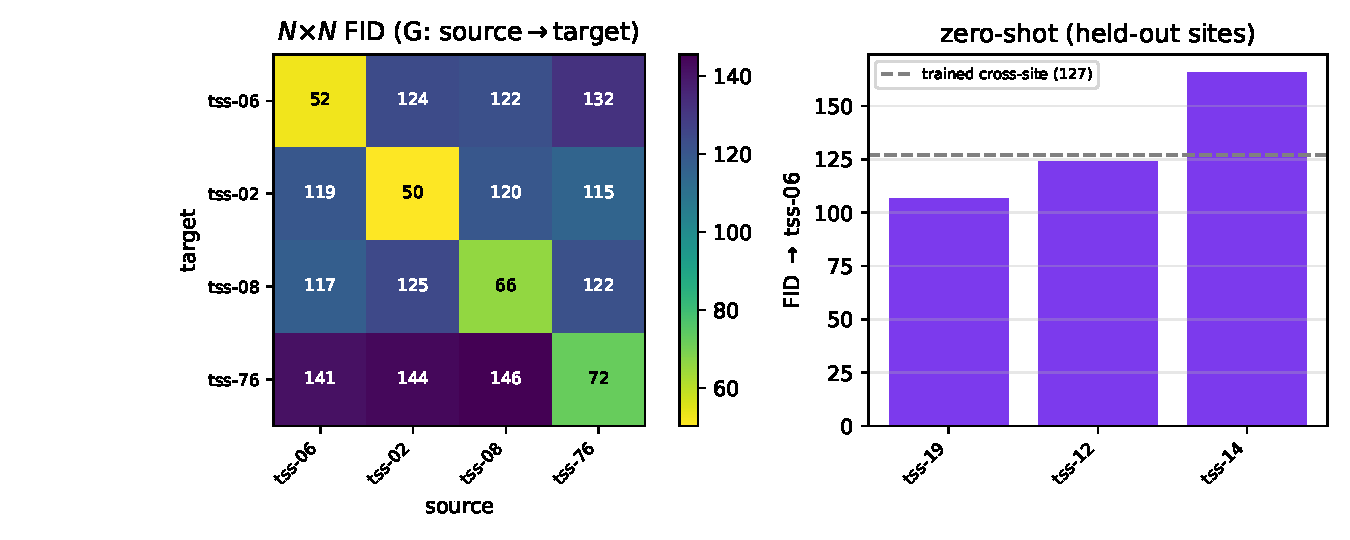
\includegraphics[width=\linewidth]{figs/fig_ext_c_matrix.pdf}
  \caption{Left: $N{\times}N$ Fr\'echet-distance matrix (source$\to$target); the
  diagonal (within-site) is markedly lower than the off-diagonal (cross-site).
  Right: zero-shot transfer of three held-out institutions to a training site
  reaches a fidelity matching the trained cross-site mean (dashed).}
  \label{fig:matrix}
\end{figure}

\paragraph{The site-style space generalizes zero-shot to held-out institutions.}
The most notable result is generalization: three institutions \emph{never seen in
training} are translated to a training site at a Fr\'echet distance ($132$ on
average) that matches the model's trained cross-site translations to that site
($127$)---one held-out site ($106$) is in fact closer than some trained sites.
The AdaIN site-style space the generator learned is therefore not a lookup table
over training sites but a continuous space into which a new institution can be
mapped, which is the property a deployable multi-site harmonizer needs.

\section{Discussion and Limitations}
\label{sec:discuss}
\paragraph{What the single model buys, honestly.}
A single $O(N)$ generator harmonizes four real institutions any-to-any and, more
importantly, extends zero-shot to unseen sites---the deployment-relevant
behavior. The honest qualifier is scale of effect: these TCGA tissue-source sites
are genuinely similar (real-image site accuracy only $0.43$), so the absolute
harmonization margins are modest, and Fr\'echet distances are inflated by the
small per-site sample. The contribution is the architecture and the
generalization property; the conservative testbed neither manufactures nor hides
a large gap.

\paragraph{Limitations and the strengthening in progress.}
(i) The site distributions are subtle and the per-site samples small; a
larger-gap, larger-$N$ cross-vendor cohort would sharpen every margin. (ii) The
headline metrics are distribution-level; a downstream glioma-segmentation transfer
(raw vs.\ harmonized, per site) is the decisive validation and is the active
extension of this work, alongside a brain-masked anatomy-SSIM metric. (iii) The
auxiliary-classifier ablation ($\lambda_{\mathrm{cls}}{=}0$) and trained pairwise /
ComBat baselines complete the design-choice and cost comparisons. (iv) A single
training seed; we report variability across the four modalities and will add seed
variance with the downstream experiments.

\section{Conclusion}
\label{sec:conclusion}
We presented a single AdaIN-conditioned, self-attention 2.5D generator that
harmonizes any-to-any across $N$ MRI acquisition sites at $O(N)$ cost, validated
on four real TCGA-GBM institutions. The model reduces within-site to roughly half
the cross-site Fr\'echet distance, drives a learned site classifier toward chance,
and---most notably---transfers zero-shot to held-out institutions at a fidelity
matching its trained translations, indicating a continuous, generalizable
site-style space. We report these effects on a deliberately conservative
real-institution testbed and identify downstream task validation as the decisive
next step.

\bibliographystyle{splncs04}
\bibliography{refs}

\end{document}
